\documentclass[11pt]{article}
\usepackage{stat110}

\titlespacing\section{0pt}{12pt plus 4pt minus 2pt}{0pt plus 2pt minus 2pt}
\titlespacing\subsection{0pt}{12pt plus 4pt minus 2pt}{0pt plus 2pt minus 2pt}
\titlespacing\subsubsection{0pt}{12pt plus 4pt minus 2pt}{0pt plus 2pt minus 2pt}

\title{Probability and Counting}
\sectionnum{1}

\author{\shira, \tim}

%\SOLUTION

\begin{document}

\maketitle

\begin{notes}

\section*{Probability}
\begin{description}
    \item[Naive Definition] - If all outcomes are equally likely, the probability of event {A} happening is:
        \[P_{\textrm{naive}}(A) = \frac{\textnormal{number of outcomes favorable to {A}}}{\textnormal{number of outcomes}}\]
        
    \item[Intersection] - Given two events {A} and {B}, $A\cap B$ means {A} \textit{and} {B}. 
    
    \item[Union] - Given two events {A} and {B}, $A\cup B$ means {A} \textit{or} {B}. 
    
    \item[Complement] - Given an event {A}, $A^C$ is called A's complement, and means when "A does \textit{not} occur", meaning everything that's not in {A}.
        
    \item[De Morgan's Laws] - A useful identity that can make calculations easier by relating unions to intersections. Analogous results hold with more than two sets.
           \begin{align*} 
        ({A} \cup { B})^c = {A^c} \cap { B^c} \\
        ({A} \cap {B})^c = { A^c} \cup { B^c}
           \end{align*}

\begin{minipage}{\linewidth}
            \centering
           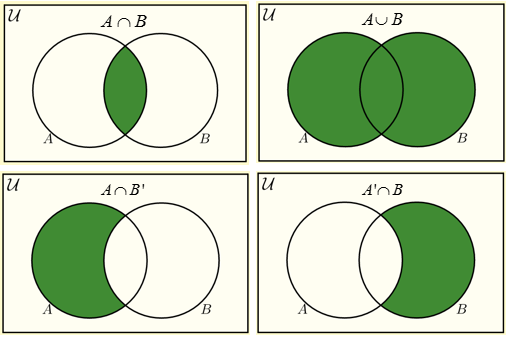
\includegraphics[width=3in]{venn.png}
        \end{minipage}
        \newline
    \item[Principle of Inclusion-Exclusion] - For any events $A_1 ,\dots , A_n$, $$P(\bigcup_{i=1}^n A_i) = \sum_i P(A_i) -\sum_{i<j} P(A_i\cap A_j) + \dots + (-1)^{n+1} P(A_1\cap\dots\cap A_n)$$
    In the small cases that we will usually deal with, this can be written as:
    \begin{align*} 
    P(A \cup B) &= P(A) + P(B) - P(A \cap B) \\
  P(A \cup B \cup C) &= P(A) + P(B) + P(C) \\
&\quad - P(A \cap B) - P(A \cap C) - P(B \cap C) \\
&\quad + P(A \cap B \cap C).
   \end{align*}
\end{description}

\section*{Counting}
\begin{description}
	\item[Multiplication Rule] - If we have $n$ decisions to make and the $j$-th decision has $r_j$ outcomes, then the total number of potential outcomes is $r_1\cdot r_2\cdot\dots\cdot r_{n-1}\cdot r_n$ 
	
	\begin{minipage}{\linewidth}
            \centering
    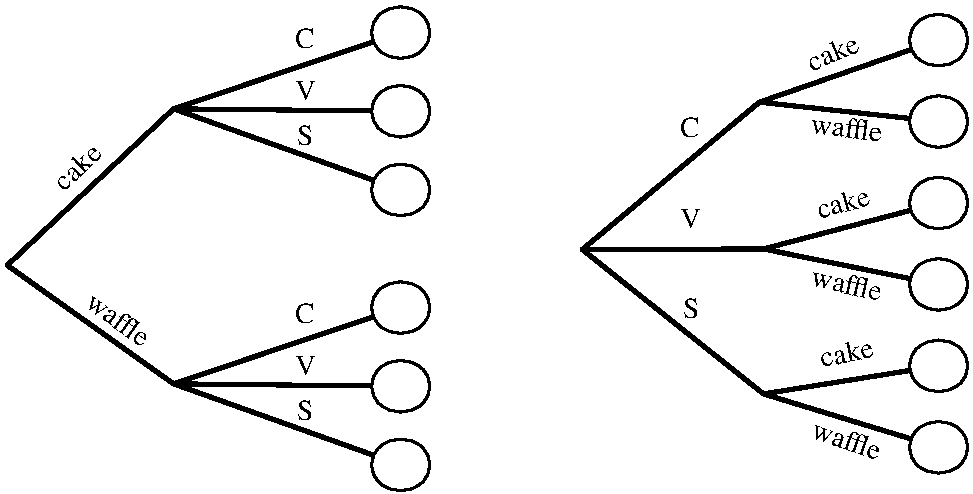
\includegraphics[width=4in]{icecream.pdf}
        \end{minipage}

	\item[Binomial Coefficient Formula] -  For $k\leq n$, we have $$ \binom{n}{k} = \frac{n(n-1)\dots(n-k+1)}{k!} = \frac{n!}{k!(n-k)!} $$ 
	$$\binom{n}{k} = \binom{n}{n-k}$$
	\item[Binomial Theorem] - $$(x+y)^n=\sum_{k=0}^n \binom{n}{k}x^k y^{n-k}$$ 
	\item[Factorial] - The number of ways to order $n$ objects is given as $$n! = n\cdot(n-1)\cdot\dots\cdot2\cdot1$$
	\item[Sampling Table] - 
	The sampling table gives the number of possible samples of size $k$ out of a population of size $n$, under various assumptions about how the sample is collected. 
        \begin{table}[H]
        \begin{center}
              \setlength{\extrarowheight}{7pt}
            \begin{tabular}{r|cc}
                 & \textbf{Order Matters} & \textbf{Order Doesn't Matter} \\ \hline
                \textbf{With Replacement} & $\displaystyle n^k$ & $\displaystyle{\binom{n+k-1}{k}}$ \\
                \textbf{Without Replacement} & $\displaystyle\frac{n!}{(n - k)!}$ & $\displaystyle{n \choose k}$
            \end{tabular}
        \end{center}
        \end{table}

\end{description}
\end{notes}

\newpage
\section*{Practice Problems}
\begin{exercise}{Story Proof Practice}
Story proofs are a fundamental and useful way that we will go about proving important results, especially later in the course. To that end, provide story proofs for each of the following results:

\begin{enumerate}
    \item
    $$\sum_{k=0}^n {n \choose k } = 2^n$$
    \item 
    $${n \choose k} + {n \choose k-1} = 
    {n+1 \choose k}$$
    \item 
    $$\frac{n!}{(n-k)!k!} = \frac{n \cdot (n-1)
    \dotsm (n-k+1)}{k\cdot (k-1)\dotsm 1}$$
\end{enumerate}
\end{exercise}

\begin{solution}{4}
\begin{enumerate}
    \item Suppose we want to figure out all possible
    teams, of any size, we can make from $n$ people. \\
    
    (RHS) Since each person is either on or off
    the team, there are $2^n$ possible teams. You
    could view this as a binary sequence, where
    each person is either a 1 or 0, leading to 
    $2^n$ total possible sequences. \\
    
    (LHS) ${n \choose k}$ represents the number
    of teams of size $k$ we can make from $n$ people.
    ${n \choose 0}$ represents all teams of size 0,
    ${n \choose 1}$ represents all teams of size 1,
    and so on. Therefore, $\sum_{k=0}^n {n \choose k}$ represents all possible teams. 
    \item Suppose we have a group of $n$ people and
    a celebrity, and we have to select a committee
    of $k$ people.\\
    
    (RHS) The straightforward way is to just 
    choose $k$ people from the group of $n+1$, 
    giving us ${n+1 \choose k}$ possible 
    committees.\\
    
    (LHS) Suppose we must have the celebrity on the 
    committee. Then there are ${n \choose k-1}$ 
    ways to choose who else will be on the committee.
    Also, suppose that we don't want to have
    the celebrity on the committee. Then there
    are ${n \choose k}$ ways to choose who 
    is on the committee. This gives us a total
    of ${n \choose k-1} + {n \choose k}$ ways
    to pick the committee. 
    \item Recall that these two expressions both
    represent ${n \choose k}$ or the number 
    of ways to choose a committee of size $k$ from
    $n$ people. \\
    
    (LHS) We first permute the $n$ people and then
    select the first $k$ people in the
    permutation. While there $n!$ total permutations,
    we must deal with the overcounting within
    the committee and the people not selected
    for the committee. The $k$ people in the 
    committee can be ordered in $k!$ ways 
    and the people not in the committee can
    be ordered in $(n-k)!$ ways, which indicates that we have overcounted by a factor of $k!(n-k)!$.
    Therefore, we observe that 
        $${n \choose k} = \frac{n!}{k!(n-k)!}$$
    (RHS) Alternatively, we can select the 
    committee directly without permuting the $n$ 
    people. We have $n$ choices for the first
    person on the committee, $n-1$ choices 
    for the second person, and so on. We know
    by the multiplication rule that there
    are $n \cdot (n-1) \dotsm (n-k+1)$ committees
    of size $k$. However, since order doesn't matter
    within the committee, we have overcounted
    by a factor of $k!$. Therefore, we observe
    that
        $${n\choose k} = \frac{n \cdot (n-1) \dotsm (n-k+1)}{k \cdot(k-1)\dots1}$$
\end{enumerate}
\end{solution}

\begin{exercise}{So Many Committees}
An organization with $2n$ people consists of $n$ married couples. A committee of size $k$ is selected, with all possibilities equally likely. Find the probability that there are exactly $j$ married couples within the committee.
\end{exercise}

\begin{solution}{2.5}
We know that there are ${2n \choose k}$ total committees possible. Next, we know there must be exactly $j$ couples within the committee, and there are ${n \choose j}$ ways to decide which couples will be on the committee. Now, it is simply a matter of ensuring that the rest of the $k-2j$ spots are filled with non-couples. \\

We have ${n-j \choose k-2j}$ ways to choose couples from the remaining couples. Then, within each of the $k-2j$ pairs, we only need one partner to be on the committee, which means there are $2^{k-2j}$ ways to choose which partner in each couple is on the committee. \\

Therefore, the probability that there are exactly $j$ married couples within the committee is 
    $$\frac{{n \choose j} {n-j \choose k-2j} 2^{k-2j}}{{\binom{2n} {k}}}$$
\end{solution}

\begin{exercise}{Counting Chocolates}
Suppose you have 15 chocolate bars and 10 section students. How many ways can you distribute the chocolate bars to your section students, in each of the following scenarios? 
\begin{enumerate}
    \item The chocolate bars are interchangeable (i.e. it doesn't matter where 
    each particular bar goes).
    \item The chocolate bars are interchangeable, but each student must receive 
    at least one. \\
    Hint: First make sure each student gets a chocolate bar and then figure out
    what to do with the remaining 5. 
    \item The chocolate bars are not interchangeable.
    \item The chocolate bars are not interchangeable, and each student must 
    receive at least one. \\
    Hint: Consider randomly giving the chocolate bars to students and then 
    apply inclusion-exclusion.
\end{enumerate}
\end{exercise}

\begin{solution}{4}
\begin{enumerate}
    \item In this case, since order does not matter and we have replacement (in 
    the sense that a student can get multiple bars), we can view the chocolate
    bars as indistinguishable particles and students as distinguishable boxes.
    This allows us to use the Bose-Einstein value, which means there are
        $${10 + 15 -1 \choose 15} = 1307504$$
    ways to distribute the bars.
    \item If we distribute 10 chocolate bars to each of the 10 students first, then
    we only need to figure out how to distribute 5 more. We can directly apply
    Bose-Einstein again to obtain
        $${10 + 5 -1 \choose 5} = 2002$$
    Another way to view this problem visually is to line up the 15 bars. Since
    each student must receive at least one bar, we simply need to place 
    9 partitions to divide the line into 10 parts. Since there are 14 spots for
    partitions, we have 
        $${14 \choose 9} = {14 \choose 5} = 2002$$
    ways to distribute the bars.     
    \item This is simply sampling with replacement where order matters, 
    so we use the multiplication rule to get $10^{15}$.
    \item Let $X_i$ be the event that student $i$ does not receive a chocolate bar,
    and note that 
        $$P(X_1 \cap X_2 \dots \cap X_k) = \left(\frac{10-k}{10}\right)^{15}$$
    for $1 \leq k \leq 10$. Now, we are interested in the probability that at least
    one student does not receive a chocolate bar. We can first calculate this
    using inclusion-exclusion and the probability we have noted above:
        $$10\left(\frac{9}{10}\right)^{15} - {10 \choose 2}\left(\frac{8}{10}\right)^{15} + \dotsm + {10 \choose 9}\left(\frac{1}{10}\right)^{15}$$
    However, we can also use the naive definition of probability. Let $x$ be the number of ways that each student receives at least one chocolate bar. Then, the probability that at least one student does not receive a chocolate bar is simply $\frac{10^{15} - x}{10^{15}}$.\\
    
    Equating these two equations and solving for $x$, we see that the number of ways such that each student receives at least one chocolate bar is 
        $$\sum_{i=0}^9 (-1)^i {10 \choose i}(10-i)^{15}$$
\end{enumerate}
\end{solution}

\begin{exercise}{Poker Probabilities.}
Suppose we have a standard 52-card deck, from which you are dealt five cards. Compute the probability of each of the following hands:
    \begin{enumerate}
        \item A royal flush (getting 10, Jack, Queen, King, and Ace of the same suit).
        \item A flush (all of the cards are of the same suit).
        \item A straight (all five cards are in consecutive order)
        \item A three-of-a-kind (three cards show the same number, and the other two cards do not form a pair)
        \item A two-pair (two cards form a pair and another two cards form a different pair)
    \end{enumerate}
\end{exercise}

\begin{solution}{5}
We begin by noting that there are $\binom{52}{5}$ possible five card hands to start from. 
    \begin{enumerate}
        \item For each of the four suits, there is only one way to obtain a royal flush. Therefore,
        the probability is simply $\frac{4}{{52 \choose 5}} \approx 0.0002$.
        \item To obtain a flush, we must first choose a suit and then choose 5 cards from
        that suit. Therefore, the probability is $\frac{4 {13 \choose 5}}{{52 \choose 5}} \approx
        0.0019$.
        \item To obtain a straight, we first consider what the first card in our straight can be. 
        Since the five cards must be in consecutive order, we have 10 possibilities for the first
        card in our straight (that is, a straight cannot begin with a Jack, Queen, or King). However,
        once we know what the first card in the straight is, the next four cards are determined. All
        that remains is deciding which suit each card will be! Therefore, the probability is
        $\frac{10 \cdot 4^5}{{52 \choose 5}} \approx 0.0039$.
        \item We first decide which value we want our three-of-a-kind to show, which gives us 13 options.
        From there, we have a choice of which 3 of the 4 suits we want it to be. For the next two cards, 
        we require that they show different values, which means there are ${12 \choose 2}$ choices 
        for what they can be, and each of these cards can be any suit. Therefore, the probability is 
        $\frac{13{4\choose 3}{12 \choose 2}4^2}{{52\choose 5}} \approx 0.021$.\\
        
        Alternatively, for the next two cards, we know we have 48 options for the first card and 44
        options for the second card. However, we divide by 2 to deal with the overcounting. 
        \item We first decide which two values we want on each pair, which gives us ${13 \choose 2}$ options. Within each pair, we have the choice of two suits, or ${4 \choose 2}^2$ ways to choose
        the suits of the two pair. The last card must be a different value from either of the pairs, 
        and there are 11 choices with 4 choices of suit. Therefore, the probability is 
        $\frac{{13\choose 2}{4\choose 2}^2 11 \cdot 4}{{52 \choose 5}} \approx 0.047$
    \end{enumerate}
\end{solution}

\begin{exercise}{Fun Interview Problem!}
Suppose the probability of at least one car passing you at an intersection over the course of twenty minutes is given by 0.9. What is the probability that at least one car passes you over the course of five minutes? Assume that time intervals of the same length have the same probability of observing at least one car. 
\end{exercise}

\begin{solution}{2}
We know that 
    $$P(\text{at least one car in twenty minutes}) = 1 - P(\text{no cars in twenty minutes})$$ 
However, we also know that 
    $$P(\text{no cars in twenty minutes}) = (1-P(\text{at least one car in 
     five minutes}))^4$$
Plugging in 0.9 and solving, we find that the probability that at least one car passes over the course of five minutes is approximately 0.44.      
\end{solution}
\end{document}
